\documentclass[a4paper]{article}
\usepackage[14pt]{extsizes}
%%% Работа с русским языком
\usepackage{cmap}					% поиск в PDF
\usepackage{mathtext} 				% русские буквы в фомулах
\usepackage[T2A]{fontenc}			% кодировка
\usepackage[utf8]{inputenc}			% кодировка исходного текста
\usepackage[english,russian]{babel}	% локализация и переносы

%%% Дополнительная работа с математикой
\usepackage{amsfonts,amssymb,amsthm,mathtools} % AMS
\usepackage{amsmath}
\usepackage{icomma} % "Умная" запятая: $0,2$ --- число, $0, 2$ --- перечисление

%% Номера формул
%\mathtoolsset{showonlyrefs=true} % Показывать номера только у тех формул, на которые есть \eqref{} в тексте.

%% Шрифты
\usepackage{euscript}	 % Шрифт Евклид
\usepackage{mathrsfs} % Красивый матшрифт

%% Свои команды
\DeclareMathOperator{\sgn}{\mathop{sgn}}

%% Перенос знаков в формулах (по Львовскому)
\newcommand*{\hm}[1]{#1\nobreak\discretionary{}
{\hbox{$\mathsurround=0pt #1$}}{}}

%%% Работа с картинками
\usepackage{float}
\usepackage{graphicx}  % Для вставки рисунков
\graphicspath{{picturesVoprosy/}}  % папки с картинками
\setlength\fboxsep{3pt} % Отступ рамки \fbox{} от рисунка
\setlength\fboxrule{1pt} % Толщина линий рамки \fbox{}
\usepackage{wrapfig} % Обтекание рисунков и таблиц текстом

%%% Работа с таблицами
\usepackage{array,tabularx,tabulary,booktabs} % Дополнительная работа с таблицами
\usepackage{longtable}  % Длинные таблицы
\usepackage{multirow} % Слияние строк в таблице

\usepackage{cite}
\usepackage{csquotes}


%%% Заголовок
\author{Катнов Артем}
\title{Курсовая работа по теме: \\ Численное моделирование динамики частиц дроби в рудоразмольной мельнице методом дискретных элементов}
\date{\today}

\usepackage[left=3cm,right=1.5cm,top=2cm,bottom=2cm]{geometry}
\linespread{1.5}
%\parindent=1.25cm
%\oddsidemargin=4.6mm
%\textwidth=16cm
%\headheight=0cm
%\headsep=0cm
%\topmargin=-1cm
%\textheight=25.7cm

%\usepackage{caption}
%\usepackage{flafter}
%\usepackage{footmisc}

\usepackage{xcolor}
\usepackage{hyperref}
% цвета для гиперссылок
\definecolor{linkcolor}{HTML}{0000FF} % цвет ссылок
\definecolor{urlcolor}{HTML}{0000FF} % цвет гиперссылок
\hypersetup{linkcolor=linkcolor, urlcolor=urlcolor, colorlinks=true}

\usepackage{cleveref}
%\usepackage{underscore}
%\usepackage{etoolbox}
%\usepackage{lastpage}
%\usepackage{titlesec}
%\usepackage{flafter}
%\usepackage{color}
%\usepackage{mfirstuc}
%\usepackage{nomencl}
%\usepackage{iftex}

\begin{document}

\selectfont
\newpage

\section{В какой точке пространства должны появиться новвые шары?}

\subsection{Описание}
Проблема в том, что большинство шаров находятся в состоянии плотной упаковки \ref{pic:upak}
\begin{figure}[h!]
	\centering
	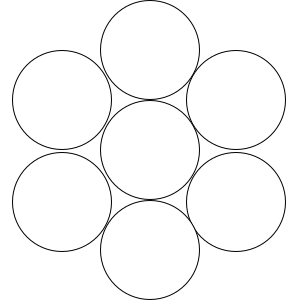
\includegraphics[width=0.4\textwidth]{Component1}
	\caption{Плотная упаковка}
	\label{pic:upak}
\end{figure} 

При разбиении должно происходить сохранение массы. 
Следовательно сумма кубов радиусов(так как у нас шары, а не диски) новых шаров должна давать куб радиуса изначального шара.
Как это выглядит при разном количестве новых шаров визуально показано на рисунках ниже.

\begin{figure}[h!]
	\centering
	\includegraphics[width=0.4\textwidth]{Component2}
	\label{pic:2balls}
	\caption{}
\end{figure} 

\begin{figure}[h!]
	\centering
	\includegraphics[width=0.4\textwidth]{Component3}
	\label{pic:3balls}
	\caption{}
\end{figure} 

\begin{figure}[h!]
	\centering
	\includegraphics[width=0.4\textwidth]{Component4}
	\label{pic:4balls}
	\caption{}
\end{figure} 

\subsection{Проблема 1}

Шары очень сильно накладываются друг на друга в данной модели.
Я боюсь что это может привести к неадекватному поведению программы.
Они очень сильно неконтролируемо могут начать разлетаться.

\textbf{Возможное костыльное решение.} 	Можно поставить ограничение на скорость, но это будет влиять на работу программы.

\textbf{Возможное честное решение.} Можно реализовать сложные фигуры, но это мне кажется довольно сложным и не факт, что я одно это успею сделать к диплому.

\subsection{Проблема 2}

Так как мы сохраняем массу (сумма кубов), то говорить о равенстве площади не приходится.
Это приведет к тому что визуально объем материала будет увеличиваться.
Хотя масса останется прежней.

\textbf{Возможное костыльное решение.} Можно заменить шары на диски.

\newpage

\section{Какая модель разрушения должна быть?}

1) 
Первый вариант описан в работе Альтшуля Г..
В этом случае у каждого шара есть параметр $\chi$.
Изначально он равен 0, но в тот момент когда он достигает 1 -- шар разрушается.
При контакте образуется $\Delta \chi$
\[
\begin{aligned}
\chi += \Delta \chi \\
\Delta \chi = \dfrac{1}{F_i}
\end{aligned}
\]

$F_i$ -- амплитуда силы в данном контакте (изменяющемся по синусоидальному закону).

Альтшуль Г. предлагает считать $F_i$ как $F_i = C \cdot (t_{kr})^n$ где C, n -- эмпирические коэффициенты, а $t_{kr}$ -- время проведенной в зацеплении.

Но работа моей программы предполагает что я могу найти точное значение $F_i$.
Возможно стоит этот способ несколько модифицировать и обойти без эмпирически получаемых коэффициентов.

2) 
Этот способ описан в \url{https://openbooks.itmo.ru/read_pribor/16002/16002.pdf} .

Сначала определяется энергия взаимодействия $E$.
Если $E$ превышает $E_{min}$ (которая является константой материала), то параметр материала $E_t$ увеличивается
\[
E_t += E - E_{min}
\]
Далее расчитывается вероятность распада частицы по формуле 
\[
P = 1 - \exp^{-S \cdot E_t}
\]

$S$ -- параметр прочности материала.

Если частица разрушена, то ее фрагменты генерируются по алгоритму разрушения Вороного ( \url{http://inis.jinr.ru/sl/vol1/CMC/Preparata,Sheimos,Vychislitelnaya\%20geometriya,\%201989.pdf} ).
Этот алгоритм я пока не понял (он как будто вообще про другое), а другого объяснения найти не смог.
Но насколько я понял -- этот алгоритм (в купе с парой других) позволяет спрогнозировать положение новообразованных шаров. Это бы могло решить предыдущую проблему если бы у нас в распоряжении были не только шары, но и более сложные геометрические фигуры.


\section{Какую скорость должны иметь образованные частицы?}

Пока кажется очевидным ответ что такую же как и первоначальная.

\section{Должно ли быть ограничение на минимальный радиус?}

Если его не будет то частицы будут дробиться и дробиться бесконечно.

Здесь же вопрос: должны ли исчезать достаточно маленькие частицы (как это происходит в реальной мельницы)?

\end{document}